% ----------------------------------------------------------
\chapter{Introdução}
% ----------------------------------------------------------

O fornecimento de água, é um dos serviços mais essenciais a vida humana, seja para abastecer as residências, ou também, serviços públicos, indústrias, usinas hidrelétricas, produção agrícola e agropecuária, economia e meio ambiente. Fazer uma gestão eficiente da utilização dos recursos hídricos é primordial para garantir que todos esses setores continuem funcionando de forma sustentável, e é também uma questão de saúde pública. De acordo com informações do \textcite{MS_Secas}, cenários de seca afetam a produção agrícola, levando a um cenário que contribui para a desnutrição da população em geral. Além disso, a falta de água tem um efeito direto na desidratação e na transmissão de doenças uma vez que é necessário acionar fontes de água não devidamente tratadas para tentar suprir a falta de água.   

Os chamados produtores de água são sistemas de reservatórios e estruturas de captação que têm a função de armazenar, regular e distribuir o recurso hídrico para os diferentes usos. Além disso, esses produtores garantem o fornecimento contínuo, e são sistemas que desempenham papel estratégico na segurança hídrica, pois permitem equilibrar a oferta de água frente às variações climáticas, às oscilações sazonais de precipitação e às crescentes demandas da população e da economia. Dessa forma, atuam como elementos fundamentais na gestão integrada dos recursos hídricos, contribuindo para a sustentabilidade ambiental e para a manutenção da qualidade de vida. 

De acordo com a \textcite{ANA_Cantareira}, o Sistema Cantareira (SC), é um dos maiores produtores de água do mundo, se posicionando como o maior entre os sistemas que abastecem a Região Metropolitana de São Paulo (RMSP). Com uma capacidade de volume útil de aproximadamente 980 bilhões de litros e produção de vazão média de 33m³/s, o sistema é responsável por abastecer cerca de 46\% da população da RMSP.  O Sistema Cantareira é formado pelos reservatórios Jaguari, Jacareí, Cachoeira, Atibainha e Paiva Castro, interligados por canais e túneis subterrâneos. Além dessa rede de conexão, o sistema conta com uma estação elevatória que bombeia a água para superar a Serra da Cantareira e com uma estação de tratamento, responsável pela preparação antes da distribuição e abastecimento. Os reservatórios recebem água proveniente de diversas bacias hidrográficas, alimentados pelas vazões dos mananciais, rios, lençóis freáticos e pela precipitação, garantindo o suprimento contínuo ao sistema. A \autoref{fig:Fig_1} a seguir, retrata visualmente o funcionamento do Sistema Cantareira. 

\begin{figure}[H]
	\centering
	\caption{Esquema Geral do Funcionamento do Sistema Cantareira.}
	\label{fig:Fig_1}
	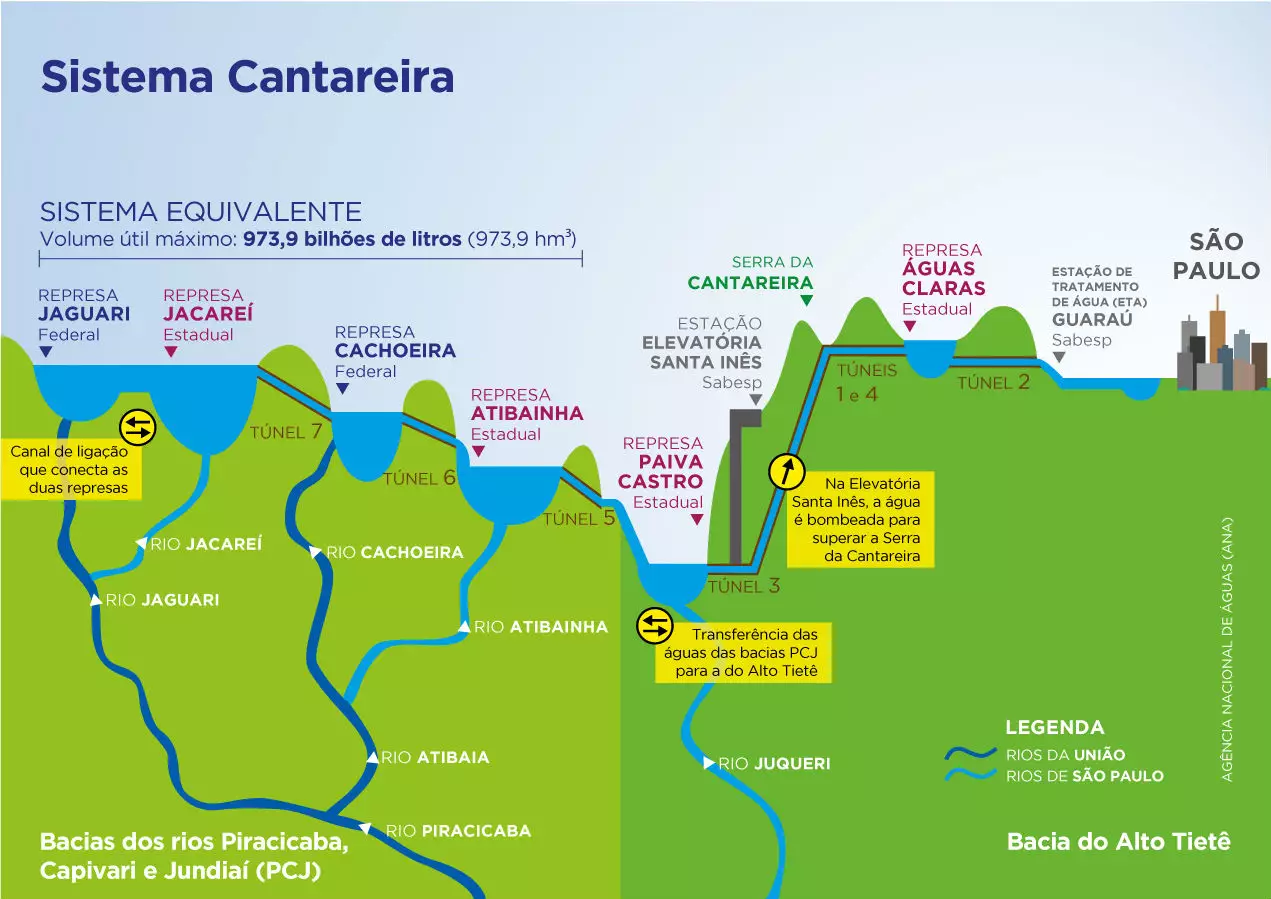
\includegraphics[width=0.8\textwidth,keepaspectratio]{figuras/imagem1.png}
	\fonte{Agência Nacional de Águas e Saneamento Básico (ANA) (2023).}
\end{figure}

A gestão do sistema é de responsabilidade da Agência Nacional de Águas (ANA) e do Departamento de Águas e Energia Elétrica do Estado de São Paulo (DAEE), já a operação do sistema é feita pela Companhia de Saneamento Básico de São Paulo (SABESP), sendo essa a responsável por observar e notificar a necessidade de operações emergenciais em casos excepcionais. Entre as diversas ferramentas de controle utilizadas pela SABESP no Sistema Cantareira, destaca-se a coleta diária de dados da situação operacional — como volumes, vazões e precipitação. Essa atividade representa apenas uma parte do conjunto de ações de monitoramento, mas no escopo deste trabalho, é a principal, uma vez que é o insumo para formar nossa base de dados.  

Os dados coletados permitem acompanhar a situação dos reservatórios, bem como a entrada e saída de água no sistema. Por meio dessas informações, torna-se possível construir análises temporais que evidenciem tendências e padrões de comportamento das variáveis envolvidas. A utilização de séries históricas de volumes, vazões e precipitação possibilita não apenas identificar cenários críticos de forma antecipada, mas também propor medidas de racionalização que contribuam para evitar ou mitigar os efeitos da escassez. Nossa proposta de trabalho concentra-se justamente nesse potencial: oferecer uma ferramenta de apoio às decisões de disponibilização de água pela SABESP, colaborando para reduzir os impactos sociais e econômicos que a má gestão desse recurso essencial pode ocasionar. 

\section{Objetivos Gerais}

\begin{itemize}
    \item Contribuir para a melhoria da gestão dos recursos hídricos no Sistema Cantareira, por meio da análise temporal de dados operacionais, visando antecipar cenários críticos e apoiar decisões de racionalização no abastecimento. 
    \item Utilizar de maneira prática os conhecimentos teóricos aprendidos ao longo do curso e criar uma solução de ciência de dados com arquitetura produtiva. 
\end{itemize}

\subsection{Objetivos Específicos}

\begin{itemize}
    \item Desenvolver uma ferramenta capaz de organizar e analisar séries temporais de variáveis operacionais (volumes e vazões).
    \item Identificar padrões e tendências que permitam prever situações de escassez ou risco no abastecimento.
    \item Propor visualizações e indicadores que facilitem a interpretação dos dados pelos gestores.
\end{itemize}